\begin{figure}[H]
    \centering



\tikzset{every picture/.style={line width=0.75pt}} %set default line width to 0.75pt        

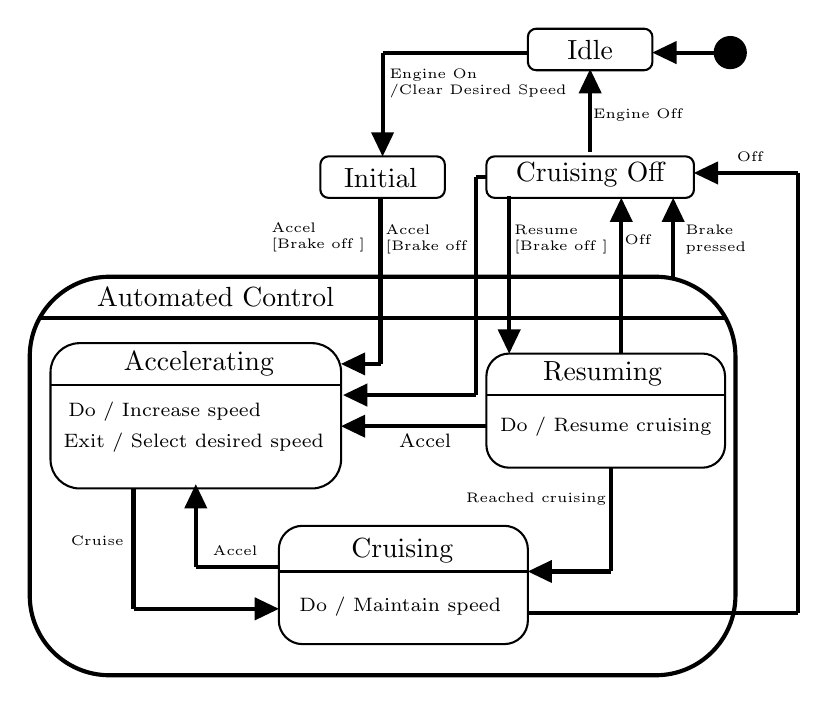
\begin{tikzpicture}[x=0.75pt,y=0.75pt,yscale=-1,xscale=1]
%uncomment if require: \path (0,423); %set diagram left start at 0, and has height of 423

%Rounded Rect [id:dp6662432613291265] 
\draw   (350,77.5) .. controls (350,75.29) and (351.79,73.5) .. (354,73.5) -- (406,73.5) .. controls (408.21,73.5) and (410,75.29) .. (410,77.5) -- (410,89.5) .. controls (410,91.71) and (408.21,93.5) .. (406,93.5) -- (354,93.5) .. controls (351.79,93.5) and (350,91.71) .. (350,89.5) -- cycle ;
%Rounded Rect [id:dp6675663074581135] 
\draw   (330,139) .. controls (330,136.79) and (331.79,135) .. (334,135) -- (426,135) .. controls (428.21,135) and (430,136.79) .. (430,139) -- (430,151) .. controls (430,153.21) and (428.21,155) .. (426,155) -- (334,155) .. controls (331.79,155) and (330,153.21) .. (330,151) -- cycle ;
%Rounded Rect [id:dp4902980476857408] 
\draw   (250,139) .. controls (250,136.79) and (251.79,135) .. (254,135) -- (306,135) .. controls (308.21,135) and (310,136.79) .. (310,139) -- (310,151) .. controls (310,153.21) and (308.21,155) .. (306,155) -- (254,155) .. controls (251.79,155) and (250,153.21) .. (250,151) -- cycle ;
%Rounded Rect [id:dp04982037628337932] 
\draw  [line width=1.5]  (110,231.4) .. controls (110,210.19) and (127.19,193) .. (148.4,193) -- (411.6,193) .. controls (432.81,193) and (450,210.19) .. (450,231.4) -- (450,346.6) .. controls (450,367.81) and (432.81,385) .. (411.6,385) -- (148.4,385) .. controls (127.19,385) and (110,367.81) .. (110,346.6) -- cycle ;
%Straight Lines [id:da7764377667791469] 
\draw [line width=1.5]    (115,213) -- (445,213) ;
%Rounded Rect [id:dp3592571098130719] 
\draw   (120,239) .. controls (120,231.27) and (126.27,225) .. (134,225) -- (246,225) .. controls (253.73,225) and (260,231.27) .. (260,239) -- (260,281) .. controls (260,288.73) and (253.73,295) .. (246,295) -- (134,295) .. controls (126.27,295) and (120,288.73) .. (120,281) -- cycle ;
%Straight Lines [id:da12221010491803885] 
\draw    (120,245) -- (260,245) ;
%Straight Lines [id:da7923623652305394] 
\draw [line width=1.5]    (380,133) -- (380,97) ;
\draw [shift={(380,93)}, rotate = 450] [fill={rgb, 255:red, 0; green, 0; blue, 0 }  ][line width=0.08]  [draw opacity=0] (11.61,-5.58) -- (0,0) -- (11.61,5.58) -- cycle    ;
%Straight Lines [id:da4788139730465273] 
\draw [line width=1.5]    (280,85) -- (280,131) ;
\draw [shift={(280,135)}, rotate = 270] [fill={rgb, 255:red, 0; green, 0; blue, 0 }  ][line width=0.08]  [draw opacity=0] (11.61,-5.58) -- (0,0) -- (11.61,5.58) -- cycle    ;
%Straight Lines [id:da6292308218465252] 
\draw [line width=1.5]    (280,85) -- (350,85) ;
%Straight Lines [id:da0875450823970263] 
\draw [line width=1.5]    (279,155) -- (279,235) ;
%Straight Lines [id:da699195185218056] 
\draw [line width=1.5]    (279,235) -- (264,235) ;
\draw [shift={(260,235)}, rotate = 360] [fill={rgb, 255:red, 0; green, 0; blue, 0 }  ][line width=0.08]  [draw opacity=0] (11.61,-5.58) -- (0,0) -- (11.61,5.58) -- cycle    ;
%Rounded Rect [id:dp8856700522665595] 
\draw   (330,241) .. controls (330,234.92) and (334.92,230) .. (341,230) -- (434,230) .. controls (440.08,230) and (445,234.92) .. (445,241) -- (445,274) .. controls (445,280.08) and (440.08,285) .. (434,285) -- (341,285) .. controls (334.92,285) and (330,280.08) .. (330,274) -- cycle ;
%Straight Lines [id:da9945138562971891] 
\draw    (330,250) -- (445,250) ;
%Straight Lines [id:da6156951818554592] 
\draw [line width=1.5]    (330,265) -- (264,265) ;
\draw [shift={(260,265)}, rotate = 360] [fill={rgb, 255:red, 0; green, 0; blue, 0 }  ][line width=0.08]  [draw opacity=0] (11.61,-5.58) -- (0,0) -- (11.61,5.58) -- cycle    ;
%Rounded Rect [id:dp5701769675760315] 
\draw   (230,324.4) .. controls (230,318.1) and (235.1,313) .. (241.4,313) -- (338.6,313) .. controls (344.9,313) and (350,318.1) .. (350,324.4) -- (350,358.6) .. controls (350,364.9) and (344.9,370) .. (338.6,370) -- (241.4,370) .. controls (235.1,370) and (230,364.9) .. (230,358.6) -- cycle ;
%Straight Lines [id:da16447218181580947] 
\draw    (230,335) -- (350,335) ;
%Straight Lines [id:da8763315052436695] 
\draw [line width=1.5]    (190,333) -- (190,297) ;
\draw [shift={(190,293)}, rotate = 450] [fill={rgb, 255:red, 0; green, 0; blue, 0 }  ][line width=0.08]  [draw opacity=0] (11.61,-5.58) -- (0,0) -- (11.61,5.58) -- cycle    ;
%Straight Lines [id:da04338392142075098] 
\draw [line width=1.5]    (190,333) -- (230,333) ;
%Straight Lines [id:da5695037590069909] 
\draw [line width=1.5]    (160,353) -- (226,353) ;
\draw [shift={(230,353)}, rotate = 180] [fill={rgb, 255:red, 0; green, 0; blue, 0 }  ][line width=0.08]  [draw opacity=0] (11.61,-5.58) -- (0,0) -- (11.61,5.58) -- cycle    ;
%Straight Lines [id:da10244373323079281] 
\draw [line width=1.5]    (160,295) -- (160,353) ;
%Straight Lines [id:da8658544131618406] 
\draw [line width=1.5]    (390,335) -- (354,335) ;
\draw [shift={(350,335)}, rotate = 360] [fill={rgb, 255:red, 0; green, 0; blue, 0 }  ][line width=0.08]  [draw opacity=0] (11.61,-5.58) -- (0,0) -- (11.61,5.58) -- cycle    ;
%Straight Lines [id:da7034657843967269] 
\draw [line width=1.5]    (390,285) -- (390,335) ;
%Straight Lines [id:da5226411692819652] 
\draw [line width=1.5]    (480,143) -- (434,143) ;
\draw [shift={(430,143)}, rotate = 360] [fill={rgb, 255:red, 0; green, 0; blue, 0 }  ][line width=0.08]  [draw opacity=0] (11.61,-5.58) -- (0,0) -- (11.61,5.58) -- cycle    ;
%Straight Lines [id:da01310825459474807] 
\draw [line width=1.5]    (480,143) -- (480,355) ;
%Straight Lines [id:da8077248116651661] 
\draw [line width=1.5]    (350,355) -- (480,355) ;
%Straight Lines [id:da581938331155091] 
\draw [line width=1.5]    (420,193) -- (420,159) ;
\draw [shift={(420,155)}, rotate = 450] [fill={rgb, 255:red, 0; green, 0; blue, 0 }  ][line width=0.08]  [draw opacity=0] (11.61,-5.58) -- (0,0) -- (11.61,5.58) -- cycle    ;
%Straight Lines [id:da5646686872608353] 
\draw [line width=1.5]    (395,230) -- (395,159) ;
\draw [shift={(395,155)}, rotate = 450] [fill={rgb, 255:red, 0; green, 0; blue, 0 }  ][line width=0.08]  [draw opacity=0] (11.61,-5.58) -- (0,0) -- (11.61,5.58) -- cycle    ;
%Straight Lines [id:da777864348657342] 
\draw [line width=1.5]    (341,154) -- (341,226) ;
\draw [shift={(341,230)}, rotate = 270] [fill={rgb, 255:red, 0; green, 0; blue, 0 }  ][line width=0.08]  [draw opacity=0] (11.61,-5.58) -- (0,0) -- (11.61,5.58) -- cycle    ;
%Shape: Circle [id:dp37606004244595703] 
\draw  [fill={rgb, 255:red, 0; green, 0; blue, 0 }  ,fill opacity=1 ] (440,85) .. controls (440,80.86) and (443.36,77.5) .. (447.5,77.5) .. controls (451.64,77.5) and (455,80.86) .. (455,85) .. controls (455,89.14) and (451.64,92.5) .. (447.5,92.5) .. controls (443.36,92.5) and (440,89.14) .. (440,85) -- cycle ;
%Straight Lines [id:da3457264380323728] 
\draw [line width=1.5]    (440,85) -- (414,85) ;
\draw [shift={(410,85)}, rotate = 360] [fill={rgb, 255:red, 0; green, 0; blue, 0 }  ][line width=0.08]  [draw opacity=0] (11.61,-5.58) -- (0,0) -- (11.61,5.58) -- cycle    ;
%Straight Lines [id:da19616464722638915] 
\draw [line width=1.5]    (325,250) -- (265,250) ;
\draw [shift={(261,250)}, rotate = 360] [fill={rgb, 255:red, 0; green, 0; blue, 0 }  ][line width=0.08]  [draw opacity=0] (11.61,-5.58) -- (0,0) -- (11.61,5.58) -- cycle    ;
%Straight Lines [id:da6702411290187669] 
\draw [line width=1.5]    (325,145) -- (325,250) ;
%Straight Lines [id:da7965543187487978] 
\draw [line width=1.5]    (325,145) -- (330,145) ;

% Text Node
\draw (380,83.5) node   [align=left] {Idle};
% Text Node
\draw (380,143.74) node   [align=left] {Cruising Off};
% Text Node
\draw (279,145.5) node   [align=left] {Initial};
% Text Node
\draw (199.5,202.5) node   [align=left] {Automated Control};
% Text Node
\draw (191.5,235) node   [align=left] {Accelerating};
% Text Node
\draw (386,239.5) node   [align=left] {Resuming};
% Text Node
\draw (289.5,325) node   [align=left] {Cruising};
% Text Node
\draw (326,100) node  [font=\tiny] [align=left] {Engine On\\/Clear Desired Speed};
% Text Node
\draw (142.5,320) node  [font=\tiny] [align=left] {Cruise};
% Text Node
\draw (209,325) node  [font=\tiny] [align=left] {Accel};
% Text Node
\draw (300.5,272) node  [font=\scriptsize] [align=left] {Accel};
% Text Node
\draw (457,135) node  [font=\tiny] [align=left] {Off};
% Text Node
\draw (366,175) node  [font=\tiny] [align=left] {Resume\\\lbrack Brake off \rbrack };
% Text Node
\draw (440.5,175) node  [font=\tiny] [align=left] {Brake\\pressed};
% Text Node
\draw (175,258) node  [font=\scriptsize] [align=left] {Do / Increase speed};
% Text Node
\draw (189,273) node  [font=\scriptsize] [align=left] {Exit / Select desired speed};
% Text Node
\draw (288.5,352) node  [font=\scriptsize] [align=left] {Do / Maintain speed};
% Text Node
\draw (387.5,265) node  [font=\scriptsize] [align=left] {Do / Resume cruising};
% Text Node
\draw (403,115) node  [font=\tiny] [align=left] {Engine Off};
% Text Node
\draw (354,300) node  [font=\tiny] [align=left] {Reached cruising};
% Text Node
\draw (249,174) node  [font=\tiny] [align=left] {Accel\\\lbrack Brake off \rbrack };
% Text Node
\draw (304,175) node  [font=\tiny] [align=left] {Accel\\\lbrack Brake off \rbrack };
% Text Node
\draw (403,175) node  [font=\tiny] [align=left] {Off};


\end{tikzpicture}
    \caption{Cruise control FSM example}
    \label{fig:fsmej}
\end{figure}